%%%%%%%%%%%%%%%%%%%%%%%%%%%%%%%%%%%%%%%%%%%%%%%%%%%%%%%%%%%%%%%%%%%%%%%%%%%
%%%%%%%%%%%%%%%%%%%%%%%%%%%%%%%%%%%%%%%%%%%%%%%%%%%%%%%%%%%%%%%%%%%%%%%%%%%
%%
%% The basic tex file for the header of all the lectures. 
%%

\documentclass{beamer}
\usetheme[hideallsubsections]{Berkeley}

\usepackage{color}
\usepackage{amsfonts}

\definecolor{myblue}{rgb}{0.25, 0, 0.75}
\definecolor{mygold}{rgb}{1,0.8,0.2}
\definecolor{gray}{rgb}{0.5, 0.5, 0.5}
\definecolor{lucia}{rgb}{0.8,0.4,0.7} 

\newcommand{\myurl}[1]{\href{http://#1}{\textcolor{gray}{\texttt{#1}}}}
\newcommand{\myem}[1]{\structure{#1}}
\newcommand{\RPack}[1]{\textcolor{gray}{\textsf{#1}}}
\newcommand{\pl}[1]{\texttt{#1}}
\newcommand{\Rcode}[1]{\texttt{#1}}
\newcommand{\Rfunction}[1]{\href{http://www.statmethods.net/search/index.asp?QU=#1&search=Search&Action=Search}{\textcolor{orange}{\textsf{#1}}}}
\newcommand{\myurlshort}[2]{\href{http://#1}{\textcolor{gray}{\textsf{#2}}}}
\newcommand{\RClass}[1]{\textcolor{mygold}{\textsf{#1}}}
\newcommand{\BIOCfunction}[1]{\textcolor{orange}{#1}}

\setbeamercolor{example text}{fg=lucia}
\setbeamertemplate{sections/subsections in toc}[ball unumbered]
\setbeamertemplate{frametitle continuation}[from second][]
\setbeamertemplate{itemize subitem}[triangle]
\setbeamertemplate{footline}[page number]
\setbeamertemplate{caption}[numbered]

\renewcommand{\footnotesize}{\fontsize{6.10}{12}\selectfont}

\def\argmax{\operatornamewithlimits{arg\,max}}
\def\argmin{\operatornamewithlimits{arg\,min}}


%%%%%%%%%%%%%%%%%%%%%%%%%%%%%%%%%%%%%%%%%%%%%%%%%%%%%%%%%%%%%%%%%%%%%%%%%%%
\title{R / Bioconductor: Curso Intensivo}

\author[]{\myem{Leonardo Collado Torres}\\
  Licenciatura en Ciencias Gen�micas, UNAM\\
  \myurl{www.lcg.unam.mx/\string~lcollado/index.php}\\
}

\date{
  Cuernavaca, M�xico\\
  Oct-Nov, 2008
}






\usepackage{Sweave}
\begin{document}

%%% set up some options for Sweave and R %%%

%%%%%%%%%%%%%%%%%%%%%%%%%%%%%%%%%%%%%%%%%%%%%%%%%%%%%%%%%%%%%%%%%%%%%%%%%%%
%%%%%%%%%%%%%%%%%%%%%%%%%%%%%%%%%%%%%%%%%%%%%%%%%%%%%%%%%%%%%%%%%%%%%%%%%%%
\begin{frame}[allowframebreaks]
  \titlepage
\end{frame}

\begin{frame}[allowframebreaks]
  \frametitle{Muestreo de poblaciones}
  \tableofcontents
\end{frame}

%%%%%%%%%%%%%%%%%%%%%%%%%%%%%%%%%%%%%%%%%%%%%%%%%%%%%%%%%%%%%%%%%%%%%%%%%%%
\section{Intro}

\begin{frame}[allowframebreaks]
  \frametitle{Descripci�n de la actividad}
  \begin{itemize}
    \item Hoy regresaremos al problema que les describ� en "letras.pdf" y aprenderemos a usar la funci�n sample.
	\item La sesi�n de hoy ser� mas bien pr�ctica y de nuevo, tendr�n que entregar un script comentado en la p�gina de Cursos\footnote{Si termina la gran mayor�a en clase, mejor!}.
  \end{itemize}
\end{frame}

\begin{frame}[allowframebreaks, fragile]
  \frametitle{\pl{sample}}
  \begin{itemize}
    \item Primero que nada, veamos los argumentos de la funci�n \BIOCfunction{sample}.
  \end{itemize}
\begin{Schunk}
\begin{Sinput}
> args(sample)
\end{Sinput}
\begin{Soutput}
function (x, size, replace = FALSE, prob = NULL) 
NULL
\end{Soutput}
\end{Schunk}
  \begin{itemize}
    \item $x$ es la poblaci�n de la cual queremos obtener una muestra. Generalmente es un vector.
	\item \emph{size} es el tama�o de nuestra muestra.
	\item \emph{replace} lo usamos para hacer un muestro con o sin reemplazo.
	  \begin{itemize}
	    \item \textquestiondown Qu� creen que sea eso?
	  \end{itemize}
	\item \emph{prob} es un vector con las probabilidades para cada elemento de nuestra poblaci�n.
  \end{itemize}
\end{frame}

\begin{frame}[allowframebreaks, fragile]
  \frametitle{Ejemplo}
  \begin{example}[Califs]
  Imaginemos que sus calificaciones son al azar y queremos obtener una muestra de como les va a ir en el pr�ximo examen. La poblaci�n es de 0 hasta 10 y el tama�o de nuestra muestra es de 20. Encontremos la calificaci�n promedio.
  \begin{enumerate}
    \item \textquestiondown Qu� pasa si las probabilidades son iguales?
	\item \textquestiondown Y si nuestro vector \pl{prob} es igual a (.005, .008, .012, .015, .05, .1, .126, .129, .25, .18, .125) ?
  \end{enumerate}
  \end{example}
\end{frame}

\begin{frame}[allowframebreaks, fragile]
  \frametitle{Soluci�n}
  \begin{itemize}
  \item Por sencillez, guardaremos los resultados en los objetos $x$ y $y$.
\begin{Schunk}
\begin{Sinput}
> x <- sample(x = 0:10, size = 20, 
+     replace = T)
> y <- sample(x = 0:10, size = 20, 
+     replace = T, prob = c(0.005, 
+         0.008, 0.012, 0.015, 0.05, 
+         0.1, 0.126, 0.129, 0.25, 
+         0.18, 0.125))
\end{Sinput}
\end{Schunk}
\begin{Schunk}
\begin{Sinput}
> table(x)
> table(y)
\end{Sinput}
\end{Schunk}
  \end{itemize}
\end{frame}

\begin{frame}[allowframebreaks, fragile]
  \frametitle{Nuestros resultados}
  \begin{itemize}
    \item Veamos los datos en formato de tabla.
% latex table generated in R 2.8.0 by xtable 1.5-4 package
% Tue Mar 17 19:33:22 2009
\begin{table}[ht]
\begin{center}
\begin{tabular}{rrrrrrrrrrr}
  \hline
 & 0 & 1 & 2 & 3 & 5 & 6 & 7 & 8 & 9 & 10 \\
  \hline
1 &   1 &   1 &   4 &   2 &   3 &   3 &   1 &   1 &   1 &   3 \\
   \hline
\end{tabular}
\caption{Califs 1er caso}
\end{center}
\end{table}% latex table generated in R 2.8.0 by xtable 1.5-4 package
% Tue Mar 17 19:33:22 2009
\begin{table}[ht]
\begin{center}
\begin{tabular}{rrrrrrr}
  \hline
 & 4 & 6 & 7 & 8 & 9 & 10 \\
  \hline
1 &   3 &   4 &   2 &   4 &   3 &   4 \\
   \hline
\end{tabular}
\caption{Califs 2ndo caso}
\end{center}
\end{table}  \end{itemize}
\end{frame}

\begin{frame}[allowframebreaks, fragile]
  \frametitle{:O}
  \begin{itemize}
  \item \textquestiondown Sali� lo que esperabamos dado nuestras probabilidades?
\begin{Schunk}
\begin{Sinput}
> mean(x)
\end{Sinput}
\begin{Soutput}
[1] 5.1
\end{Soutput}
\begin{Sinput}
> mean(y)
\end{Sinput}
\begin{Soutput}
[1] 7.45
\end{Soutput}
\end{Schunk}
  \end{itemize}
\end{frame}

%%%%%%%%%%%%%%%%%%%%%%%%%%%%%%%%%%%%%%%%%%%%%%%%%%%%%%%%%%%%%%%%%%%%%%%%%%%
\section{Problema}

\begin{frame}[allowframebreaks, fragile]
  \frametitle{La simulaci�n inicial}
  \begin{itemize}
  \item Primero que nada, lo siguiente es una simulaci�n sencilla para una poblaci�n de tama�o 50. Veamos que pasa si asumimos la misma probabilidad para todos los elementos y con tama�os de muestra diferentes: desde 1 hasta 1000.
  \scriptsize
\begin{Schunk}
\begin{Sinput}
> pob <- 1:50
> res <- NULL
> for (i in 1:1000) {
+     muestra <- sample(pob, size = i, 
+         replace = T)
+     prueba <- length(unique(muestra))/length(pob)
+     if (prueba >= 1) {
+         res <- c(res, 1)
+     }
+     else {
+         res <- c(res, 0)
+     }
+ }
\end{Sinput}
\end{Schunk}
  \end{itemize}
  \normalsize
\end{frame}

\begin{frame}[allowframebreaks, fragile]
  \frametitle{Explorando res}
  \begin{itemize}
  \item Si gr�ficamos nuestros resultados, veremos algo con dos estados. 
  \item Como extra, podemos usar \BIOCfunction{lines} para marcar en el eje $Y$ el 0.95
  \scriptsize
\begin{Schunk}
\begin{Sinput}
> plot(1:1000, res, col = "blue", 
+     main = "Una simulaci�n", xlab = "Tama�o de la muestra")
> lines(x = 1:1000, y = rep(0.95, 
+     1000), col = "red")
\end{Sinput}
\end{Schunk}
  \end{itemize}
  \normalsize
\end{frame}

\begin{frame}[fragile]
  \frametitle{1era simulaci�n}
  \begin{figure}[htbp] 
  \begin{centering}   
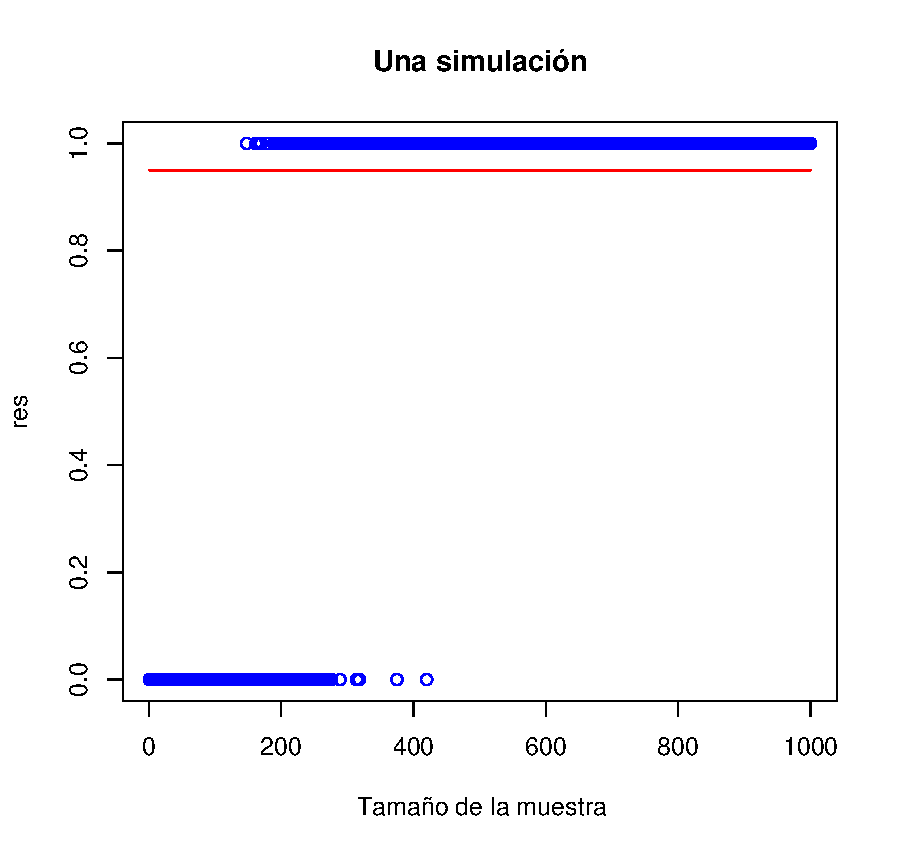
\includegraphics{plots2/sample-009}
  \end{centering} 
  \end{figure}
\end{frame}

\begin{frame}[allowframebreaks]
  \frametitle{Problema}
  \begin{itemize}
    \item Bas�ndose en la simulaci�n anterior, quiero que hagan 100 simulaciones para una poblaci�n de tama�o 10 y con probabilidades iguales.
    \item Cada simulaci�n debe explorar tama�os de muestra desde 1 hasta 100.
    \item Hagan una sola gr�fica donde resuman sus resultados con la l�nea en el 0.95 en el eje $Y$.
  \end{itemize}
\end{frame}

\begin{frame}[allowframebreaks]
  \frametitle{Tips}
  \begin{itemize}
    \item Almacenen sus resultados en una matriz \footnote{Pueden llenarla con 0s o \pl{NA}} en vez de en un vector nulo.
    \item Utilicen dos ciclos para llenar su matriz. Ya les di una \alert{super} ayuda con los 0s y 1s.
    \item Como tienen que resumir sus 100 simulaciones en una gr�fica, saquen la \_ \_ \_ \_ \_ .
  \end{itemize}
\end{frame}

%%%%%%%%%%%%%%%%%%%%%%%%%%%%%%%%%%%%%%%%%%%%%%%%%%%%%%%%%%%%%%%%%%%%%%%%%%%
\section{Soluci�n}

\begin{frame}[allowframebreaks, fragile]
  \frametitle{C�digo}
  \begin{itemize}
  \item Usando los elementos que les dije en los "Tips", obtenemos esto:
  \scriptsize
\begin{Schunk}
\begin{Sinput}
> pob <- 1:10
> res <- matrix(0, 100, 100)
> for (i in 1:100) {
+     for (j in 1:100) {
+         muestra <- sample(pob, 
+             size = j, replace = T)
+         prueba <- length(unique(muestra))/length(pob)
+         if (prueba >= 1) {
+             res[i, j] <- 1
+         }
+     }
+ }
\end{Sinput}
\end{Schunk}
  \normalsize
  \end{itemize}
\end{frame}

\begin{frame}[allowframebreaks, fragile]
  \frametitle{La gr�fica}
  \begin{itemize}
  \item El c�digo para la gr�fica es casi el mismo ^^. Noten el uso de \BIOCfunction{colMeans}.
  \scriptsize
\begin{Schunk}
\begin{Sinput}
> plot(1:100, colMeans(res), col = "blue", 
+     main = "100 simulaciones", 
+     xlab = "Tama�o de la muestra", 
+     ylab = "Media de las 100 simulaciones")
> lines(x = 1:100, y = rep(0.95, 
+     100), col = "red")
\end{Sinput}
\end{Schunk}
  \normalsize
  \end{itemize}
\end{frame}

\begin{frame}[fragile]
  \frametitle{Gr�fica final}
  \begin{figure}[htbp] 
  \begin{centering}   
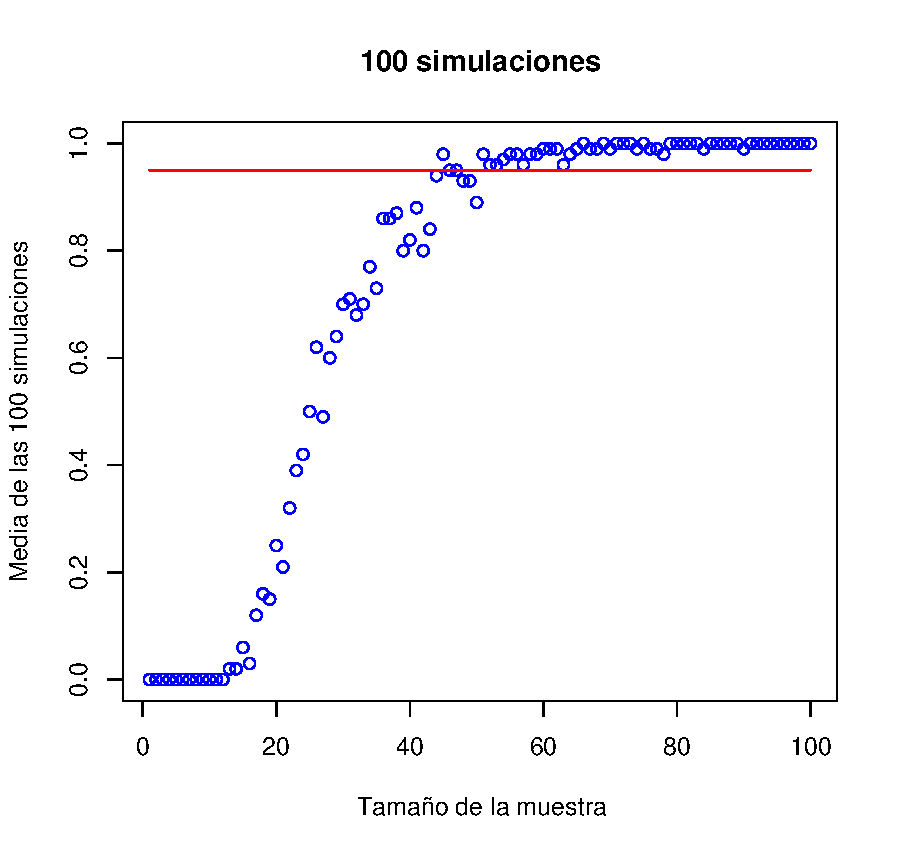
\includegraphics{plots2/sample-012}
  \end{centering} 
  \end{figure}
\end{frame}

%%%%%%%%%%%%%%%%%%%%%%%%%%%%%%%%%%%%%%%%%%%%%%%%%%%%%%%%%%%%%%%%%%%%%%%%%%%

\end{document}
